%ha med dette her
\documentclass[titlepage]{article}
\usepackage[norsk]{babel}
\usepackage[utf8]{inputenc}
\usepackage{parskip}
\usepackage{pdfpages}
%\usepackage[latin1]{inputenc}
%\usepackage{graphicx}
%\usepackage{float}

%---- Listings --------------
\usepackage{color}
\definecolor{light-gray}{gray}{0.95}
\usepackage{listings}
\lstset{numbers=right,
      %numberstyle=\tiny,
      %numbers=left,
      %stepnumber=2,
      literate={æ}{{\ae}}
        {Æ}{{\AE}}1
        {ø}{{\o}}1
        {Ø}{{\O}}1
        {å}{{\aa}}1
        {Å}{{\AA}}1,
      firstnumber=1,
      numberfirstline=true
     breaklines=true,
     backgroundcolor=\color{light-gray},
     numbersep=5pt,
     xleftmargin=.25in,
     xrightmargin=.25in}
     \lstset{language=Java}

%Listings brukes slikt:
%\begin{lstlisting}{insert}
%Sett inn kode her
%\end{lstlisting}
%--------------------------

%hva som skal stå på tittelsida
\author{grp 38}
\title{Øvinf D3}
\date{\today}

\begin{document}

%lager forsida
\maketitle

%man burde ha med et sammendrag

%man skal ha romertall på de innholdsfortegnelse
%før dette punktet skal man IKKE ha sidetall
\pagenumbering{roman}
\tableofcontents

%newpage gjør at du starter på neste side etterpå
\newpage

%herfra skal vi ha vanlige tall (arabiske (1,2,3,4,5...))
\pagenumbering{arabic}

%man pleier å starte med innledning
\section{Konseptuell modell}
Begrepet som Vi bruker i kalendersystemet vårt er:
kalender, avtale, møte, deltager, grupper, møteleder, møtelokale, alarm, notifikasjon/møteinnkalling, andre kalender, godta, avslå, rediger, slett, lagre og opprette avtale.

sammenhengen mellom begrepene:
\begin{itemize}
  \item kalender inneholder flere avtaler og møter, vi kan også legge til andre sin kalender.
  \item  et møte kan inneholde et vilkårlig antall deltagere eller grupper, ha et møtelokale, ha alarmer knyttet til seg og sende ut notifikasjoner til deltagere.
  \item Et møte er det samme som en avtale bare at man har invitert andre personer.
  \item  møtelederen er personene som startet møte, han har makten til å redigere og/eller slette møtet.
  \item notifikasjon er en varsel som blir send til alle deltagere når møtelederen velger det. Notifikasjoner blir automatisk sendt dersom møte endrer seg og deltagere kan godta eller avslå møtet.
  \item  Når man oppretter en avtale, så setter vi av starttidspunkt og sluttidspunktet, møtelokalet, hvem som kommer og om den skal sette en alarm, møtelederen kan etter det lagre avtalen og sende ut møteinnkalling.
  \item Gruppe kan inneholde et vilkårlig antall personer.
\end{itemize}

\newpage

\subsection{UML klassediagram}
\begin{figure}[ht!]
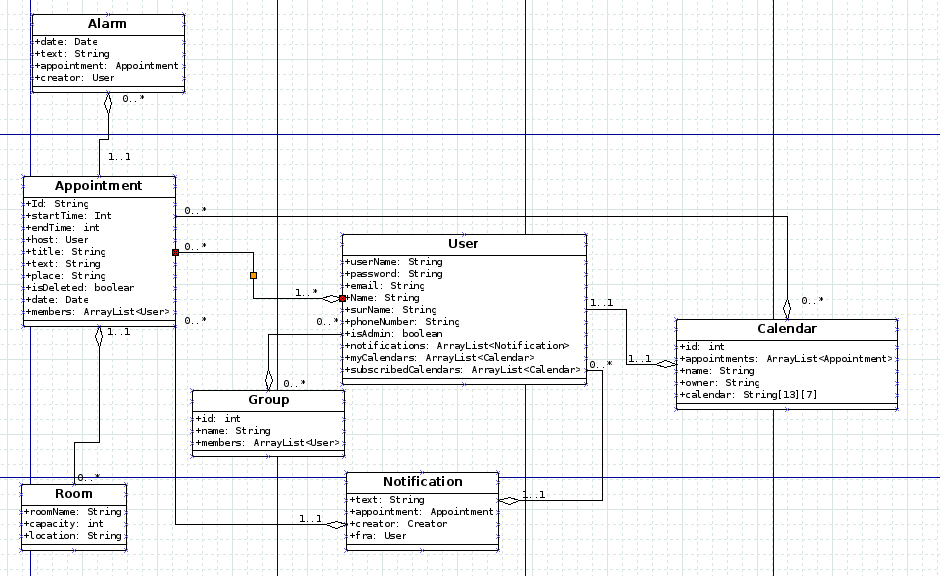
\includegraphics[width=150mm]{UML.png}
\caption{UML klassediagram}
\end{figure}

\end{document}

